\chapter{Stock returns over the FOMC Cycle Revisited }


\section{The FOMC cycle}

The FOMC (federal market open committee) meets approximately every eight weeks during the year, which results in a FOMC cycle time of approximately 7 weeks (excluding weekends) at most times since a year has 52 weeks.
The authors therefore define FOMC cycle time week dummy variables for week 0 as days -1 one to 3, week 1 as days 4 to 8,  till week 6 as days 29 to 33. Worthwhile to mention is that the authors drop 3 days which would be in FOMC cycle week 7 from their investigation and that the number of available data points for decreases for FOMC dummies (meaning 920 days in week 0, 924 days in week 2, 831 days in week 4, 120 days in week 6 for the relevant timespan from 1994 till 2016)

\label{cies19_fig2}
\begin{figure}[h]
    \centering
    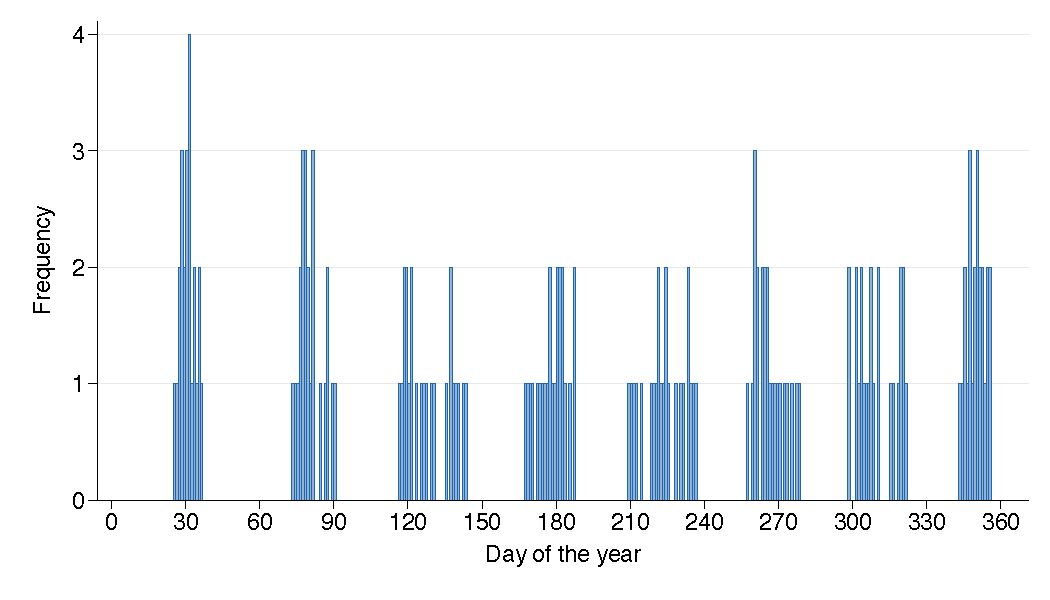
\includegraphics[width=0.75\textwidth]{figures/cies19/fig2}
    \caption{cies19 - Fig2}
\end{figure}


\section{FOMC data}

\section{Linear Regression with FOMC dummy variables}

One relevant linear regression model with FOMC cycle week as in \parencite{cieslak_stock_2019} can be defined as:
\begin{equation}
	rxpct_{i}=\hat{\beta_{0}}+D_0*\hat{\gamma_{1}}+D_1*\hat{\gamma_{2}}+\epsilon_i
\end{equation}
where
$ { \hat{\beta_{0}} } $ is the OLS-estimated intercept,
$ { \hat{\gamma_{1}}, \hat{\gamma_{2}} } $ the OLS-estimated parameters,
${ rx_{i} } $ the excess returns as calculated like in chapter 3.3., 
\begin{equation}
    D_0=
    \begin{cases}
      1, & \text{if in the 0 week within FOMC cycle time. }\\
      0, & \text{otherwise}
    \end{cases}
\end{equation}
the FOMC cycle dummy for week 0, 
\begin{equation}
    D_1=
    \begin{cases}
      1, & \text{if in the 2,4 or 6 week within FOMC cycle time. } \\
      0, & \text{otherwise}
    \end{cases}
\end{equation}
the FOMC cycle dummy for week 2,4, 6 and
$ { \epsilon_i \; \sim \; i.i.d.  \; \mathcal{N}\left(0, \sigma^2 \right) } $
are independent identically distributed OLS-estimated standard errors. 


\section{Replication with FOMC data (from 2016 onwards)}

\subsection{FOMC dummy generation}

The R Code in \texttt{generate\_fomc\_dummies\_cycle\_dummies.R}
generates FOMC week dummy variables for later estimation of the influence on FOMC meeting dates on excess stock returns.

\subsection{Data Processing}

The analysis commences with the importation and organization of two distinct datasets. 
The first dataset, identified as \texttt{fomc\_data}, is loaded from the file\\ \texttt{fomc\_week\_dummies\_1994\_nov2023.csv}. 
This dataset encompasses information related to FOMC week dummies spanning from November 1994 to November 2023. The data is sorted by date, and the sorted dataset is then saved as \texttt{d:fomc\_data}, thereby replacing any pre-existing file.

Following this, the second dataset, labeled as \texttt{us\_returns\_data}, is imported from the file \texttt{us\_returns\_df\_1994\_oct2023.csv}. This dataset contains information regarding Fama-French factors for the U.S. market, covering the period from October 1994 to October 2023. Similar to the first dataset, it undergoes sorting by date, and the sorted dataset is saved as \texttt{d:us\_returns\_data}, replacing any existing file.

To consolidate the information, a merge operation is executed using the "date" variable as the key. This operation combines the \texttt{fomc\_data} and \texttt{us\_returns\_data} datasets into a new dataset named \texttt{fed\_put\_datamerged\_data}. The merged dataset is saved as \texttt{d:fed\_put\_datamerged\_data}, effectively replacing any prior file.

Finally, a new variable named \texttt{date2} is generated by transforming the existing "date" variable into Stata date format. This conversion is carried out using the \texttt{date()} function with the "YMD" (year-month-day) format. The resulting dataset is now primed for further analysis,  incorporating information from both the FOMC week dummies and U.S. market returns datasets.

\subsection{Calculation of stock excess returns using Fama/French factors}

Excess stock returns are calculated using the Fama-French three-factor model. 

Let \(m\) represent \(1 + \text{{stock return}}\) and \(r\) denote \(1 + \text{{bill return}}\). The natural logarithms of \(m\) and \(r\) are computed as \(\ln(m)\) and \(\ln(r)\) respectively.

The 1-day excess return (\text{{ex1}}) is determined by subtracting \(r\) from \(m\) and multiplying the result by 100. This is expressed as \(\text{{ex1}} = 100 \times (m - r)\). 

The 5-day excess return (\text{{ex5}}) is computed over a rolling 5-day window, involving the product of five consecutive values of \(m\) and \(r\). The formula is given by \(\text{{ex5}} = 100 \times (m \times m_{t+1} \times m_{t+2} \times m_{t+3} \times m_{t+4} - r \times r_{t+1} \times r_{t+2} \times r_{t+3} \times r_{t+4})\).

Additionally, \(t\) represents the observation number in the dataset. 
The calculation for evaluating stock excess returns provide insight for their 
performance relative to the risk-free rate.

\subsection{Replication Results}

\begin{table}[h]
\begin{center}
\begin{adjustbox}{width=1\textwidth}

{
\def\sym#1{\ifmmode^{#1}\else\(^{#1}\)\fi}
\begin{tabular}{l*{3}{c}}
\hline\hline
            &\multicolumn{1}{c}{(1)}   &\multicolumn{1}{c}{(2)}   &\multicolumn{1}{c}{(3)}   \\
            &2014-2016 sample   &1994-2014 sample   &1994-2016 sample   \\
\hline
w\_t0        &       0.174*  &       0.138***&       0.143***\\
            &      (1.92)   &      (2.80)   &      (3.21)   \\
[1em]
w\_t2t4t6    &       0.166** &      0.0890** &      0.0990***\\
            &      (2.55)   &      (2.38)   &      (2.95)   \\
[1em]
\_cons      &     -0.0486   &     -0.0164   &     -0.0206   \\
            &     (-1.14)   &     (-0.76)   &     (-1.05)   \\
\hline
N           &         782   &        5224   &        6006   \\
significant at 1%-level (***), 5% level (**), 10% level (*)

\end{tabular}
}

\end{adjustbox}
\caption{\label{table_1} caption for table 1}
\end{center}
\end{table}


\subsection{Stock returns over the FOMC cycle from 2016 onwards}

Answer Q.: Does the stylized fact of stock excess returns are mainly achieved in FOMC even weeks (0,  2,  4,  6) from 2016 onwards still persist?

\begin{table}[h]
\begin{center}
\begin{adjustbox}{width=1\textwidth}
{
\def\sym#1{\ifmmode^{#1}\else\(^{#1}\)\fi}
\begin{tabular}{l*{4}{c}}
\hline\hline
            &\multicolumn{1}{c}{(1)}   &\multicolumn{1}{c}{(2)}   &\multicolumn{1}{c}{(3)}   &\multicolumn{1}{c}{(4)}   \\
            &   2016-2019   &   2019-2022   &   2016-2023   &   1994-2023   \\
\hline
w\_t0        &      -0.211** &     -0.0952   &      -0.125   &      0.0800** \\
            &     (-2.29)   &     (-0.57)   &     (-1.40)   &      (2.01)   \\
[1em]
w\_t2t4t6    &     -0.0487   &      0.0578   &      0.0256   &      0.0828***\\
            &     (-0.74)   &      (0.48)   &      (0.41)   &      (2.81)   \\
[1em]
\_cons      &      0.0960** &      0.0108   &      0.0434   &    -0.00622   \\
            &      (2.48)   &      (0.12)   &      (0.94)   &     (-0.34)   \\
\hline
N           &         762   &         779   &        1752   &        7772   \\
significant at 1\%-level (***), 5\% level (**), 10\% level (*)

\end{tabular}
}
\end{adjustbox}
\caption{\label{table_2} caption for table 2}
\end{center}
\end{table}

\pagebreak


% \subsection{ Stock returns over the FOMC cycle from 2016 onwards European Stock Returns}

